\documentclass{article}

% Packages
\usepackage[utf8]{inputenc}  % Encoding
\usepackage[T1]{fontenc}     % Font encoding
\usepackage{lmodern}         % Improved font rendering
\usepackage{amsmath}         % Math symbols
\usepackage{amsfonts}        % Math fonts
\usepackage{amssymb}         % Additional math symbols
\usepackage{graphicx}        % Include graphics
\usepackage{hyperref}        % Hyperlinks
\usepackage{geometry}        % Page layout
\usepackage{listings}
% \geometry{a4paper, margin=1in}
% TODO add more graphs, check grammar
% Title, author, and date
\title{Numerically Solving Navier Stokes equation with GPUs}
\author{Gašper Golob}
\date{\today}

\begin{document}

% Title
\maketitle

% Introduction
\section{Introduction}
The goal of the project is to use the GPU to accelerate the execution of two methods for 
solving the Navier Stokes equation. Specifically the two methods that are being accelerated are
the implicit and explicit variant of the artificial compressibility method.

The performance and accuracy of the GPU based versions are then tested on the 
lid driven cavity problem. The lid driven cavity problem is the case where the fluid is in 
a square case, where one of the sides induces some movement. 
The case is schematically presented in the figure \ref{fig:lid_driven_cavity}, 
from \cite{lidDriven}.
\begin{figure}[h!] 
    \centering 
    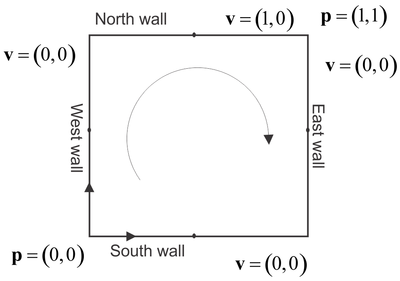
\includegraphics[width=0.6\textwidth]{lid_driven_cavity.png} 
    \caption{The schematic of the lid driven cavity problem.} 
    \label{fig:lid_driven_cavity} 
\end{figure}
It is often used to test numerical methods for fluid simulations as the velocities converge towards 
some value, which can tell us if implemented method is stable.

The methods work iteratively, where at each time step, they compute new velocities using the 
Navier Stokes equation. Afterwards they correct the pressure using an assumed pressure volume 
invariant. 

For the purposes of this project the details of solving the partial differential equations are not 
as important, since the project is mostly concerned with accelerating the solving of systems and 
various matrix operations.

The GPU versions are also compared to their base versions to gauge the level of improvement and to 
see if they remain accurate.

The project is made using C++, where the discretization of the differential equations is done using 
the medusa library \cite{medusa}. To solve linear systems and work with matrices on the CPU the 
Eigen library is used. Similarly, to work with matrices and vectors on the GPU side, 
CUDA libraries such as cuSolver, cuSparse, cuDSS and Thrust are used.
\section{Implicit method}
For the implicit version of the method we are mostly concerned with solving two linear systems.
The first involves solving a system of the form \(M_u x = b\), where the matrix \(M_u\) changes at
every time step, so we need a solver, that can quickly solve a different system on each step.

The other system \(M_p x = b\) remains unchanged between different 
iterations. It is solved up to 100 times per time step, so it makes sense to preprocess the 
matrix to improve performance.

To try and accelerate the system with the matrix \(M_u\) several solvers from different CUDA libraries 
were tried. To solve the system with the unchanging matrix \(M_p\) only one other method was attempted
as CUDA currently doesn't have too many linear system solvers, that allow for preprocessing. 

\subsection{Solvers}
All solvers are initialized using the Eigen \verb|SparseMatrix| type for sparse matrices. 
To solve a system they receive the right-hand side vector which has the Eigen type \verb|VectorXd|,
which is a dense vector whose elements have the type \verb|double|. Ultimately they return 
a vector of the same type.
\subsubsection{SparseLU solver}
The base CPU version uses the Eigen library to solve the linear systems. For both of the systems 
the SparseLU solver is used, which implements the supernodal LU factorization of the matrix, and then
solves the system using the computed triangular matrices.
\subsubsection{QR solver}
The QR solver uses the function \verb|cusolverSpDcsrlsvqr| from the cuSolverSp library. 
The function takes as arguments a sparse matrix \(A\) in the 
compressed sparse rows format alongside two dense vectors \(x\) and \(b\). It solves the 
system \(Ax=b\) on the GPU. In the background the method computes a sparse QR factorization of the matrix \(A\),
while also providing some reordering, to minimize zero fill in. For the purposes of this project,
the \verb|symrcm| reordering scheme is used.
\subsubsection{cuDSS solver}
The cuDSS solver is the main solver currently implemented in the cuDSS library. Since the matrix 
doesn't have any extra properties it uses the LDU decomposition. Same as the previous 
solver the matrix is in the CSR format, while the right-hand side and solution vectors
are dense. All the matrices and vectors are transferred to the GPU where the decomposition is 
computed and the systems are solved.
\subsubsection{RF solver}
The refactorization solver is meant to sequentially solve multiple systems of the form 
\(A x_i = b_i\) for multiple vectors \(x_i\), \(b_i\) and a fixed matrix \(A\). 

The first time 
it has to solve a system it uses the \verb|cusolverSP_lowlevel_preview| library. This library 
first computes the sparse LU decomposition (with some reordering) of the matrix and then solves the 
first system.

Afterwards the sparse LU  decomposition is extracted and passed to the \verb|cuSolverRF| library,
which can then use it to solve later systems.

The first iteration is done completely on the CPU, as the \verb|cusolverSP_lowlevel_preview| library
currently lacks GPU versions of the functions. Later, the systems are solved using the functions 
from \verb|cuSolverRF| which works on the GPU.

\subsection{Benchmarks}
To reiterate we are solving a system of the form \(M_u x = b\), which has to be solved once per time step
and \(M_p x = b\) which has to be solved multiple times per time step. The matrix \(M_u\) changes
every iteration while the matrix \(M_p\) remains fixed.

The system with the matrix \(M_u\) is accelerated using the QR and cuDSS solvers, while
the second system is only accelerated using the RF solver, as this is the only one that allows 
preprocessing. 

The execution time of the programs, when using different solvers can be seen in the
figure \ref{fig:lidDriven_time}.

We can see that the lid driven cavity version which is the reference CPU implementation 
is the slowest, except possibly right at the beginning, where there is still not that much 
parallelism. 

The second-best case is when we use the QR solver to solve the system with the matrix \(M_u\).
It starts of a bit slower than the CPU version but quickly becomes faster.

The best case is when using the cuDSS solver to solve the system with the matrix \(M_u\). For large 
enough \(N\) the performance increase seem to be about 100x, which is far better than even the QR 
solver.

The last case uses the cuDSS solver for the system with the matrix \(M_u\) and the 
RF solver for the system with the matrix \(M_p\). Unfortunately it seems that solving the  
LU system on the GPU slows down the execution, which makes some sense as solving triangular systems 
is a very sequential operation.

Regardless, it might prove useful to run the benchmarks on even larger cases, as there might be some 
performance improvements for very large \(N\). The limiting factor here might however be, that 
the LU decomposition is done on the CPU, so the setup time might take too long.
\begin{figure}[h!] 
    \centering 
    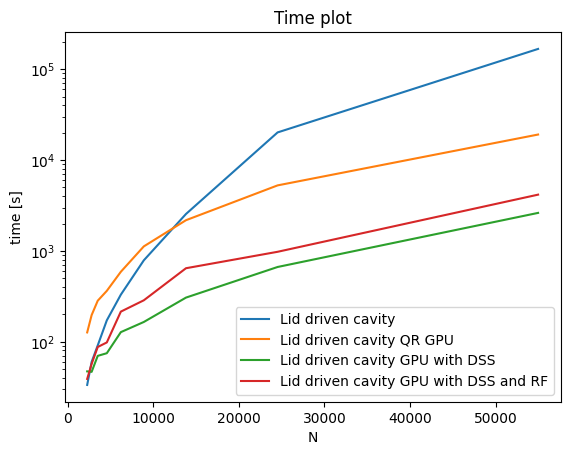
\includegraphics[width=0.8\textwidth]{lidDriven_time.png} 
    \caption{Graph of times to simulate 50 seconds of the lid driven cavity problem using
    the implicit method, for different problem sizes.} 
    \label{fig:lidDriven_time} 
\end{figure}

From the figure \ref{fig:lidDriven_convergence} at the end of the report we can see that the 
method converges toward some fixed value, which is what we expected. As a sanity check we can 
also look at \ref{fig:lidDrivenACM_cross} which tells us that the final velocities at the 
middle line match for all implementations.
\section{Explicit method}
The explicit method starts by constructing some matrices using the Medusa library. Afterwards it 
only requires matrix multiplications and some element-wise operations. This means we can transfer
all matrices and vectors to the GPU and do most of the work there. 

\subsection{Basic GPU operations and types}
For all operations sparse matrices are given in the compressed sparse row format and the vectors
are the usual dense vectors given as arrays on the GPU.
\subsubsection{VectorGPU and MatrixGPU}
These are some basic wrapper classes that convert to and from their Eigen counterparts.
Data that is passed to them is transferred to the GPU, where it can be used with other functions.
\subsubsection{Matrix multiplication}
To multiply sparse matrices with vectors the cuSparse library is used. More specifically the 
\verb|cusparseSpMV| function is used which takes a matrix in the compressed sparse rows format, 
a dense vector and returns a dense solution vector. Some multiplication data is initialized 
before the simulation as it speeds up the later multiplications. 
\subsubsection{Transforms and reduces}
For element-wise operations on dense vectors thrust's \verb|transform| and \verb|transform_reduce| 
functions are used.

The first use case is to allow element-wise vector multiplication, for which we can use 
the \verb|transform| function and the built-in \verb|multiplies| operator.

The second use case is to define a new operator \verb|axpy_functor| which is initialized using some 
value \(\alpha\) and which then for given vectors \(x\) and \(y\) computes \(y = \alpha x + y\).
The operator is again applied using the \verb|transform| function.

Another case is the definition of the operator \verb|abs_functor| which for a given vector 
computes the element-wise absolute value.

The last two operators that are defined are \verb|u_tuple_functor| and \verb|tuple_max_functor|,
which are then used with the \verb|transform_reduce| function. The \verb|u_tuple_functor| is initialized
using an array which represents a vector field. Running the functor on some set of indices
will return an array of pairs of said indices and the corresponding second coordinate values.
Then the \verb|tuple_max_functor| finds the maximum value among the values which have corresponding 
indices. This is used to find 
the maximum velocity in the \(y\) direction at the middle line of the lid driven cavity case.

Another function from Thrust that is used is \verb|max_element| which simply returns the 
maximum element of an array.
\subsection{Benchmarks}
We use the previously described functions to port the CPU code to the GPU. Additionally,
we also use CUDA streams to execute multiple operations on the graphics card at once, where 
this is possible. 

We can see the execution times of the base CPU version in comparison the GPU version on figure 
\ref{fig:lidDrivenACM_time}.
Once again the CPU version is better at the smallest values of \(N\), but it quickly becomes 
better as \(N\) grows larger.
\begin{figure}[h!] 
    \centering 
    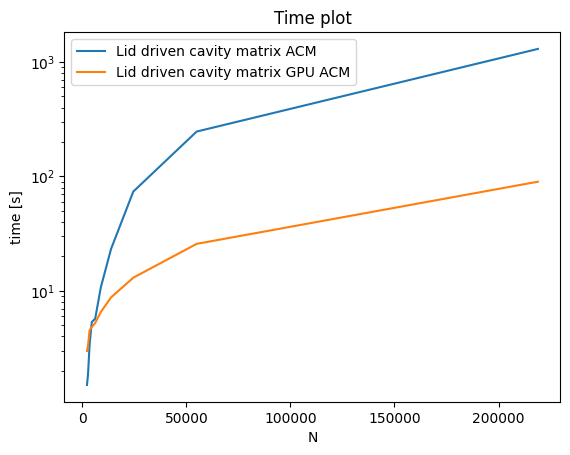
\includegraphics[width=0.8\textwidth]{lidDrivenACM_time.png} 
    \caption{Graph of times to simulate 50 seconds of the lid driven cavity problem using
    the explicit method, for different problem sizes.} 
    \label{fig:lidDrivenACM_time} 
\end{figure}

Much like for the implicit method we can also observe from \ref{fig:lidDrivenACM_convergence} that 
the methods converge towards some fixed value. Their middle line velocities also match, which we can 
see from \ref{fig:lidDrivenACM_cross}.

\section{Further work}
While the project is nearing completion there is some more work to be done. For an instance it 
would be good to benchmark the performance for some even larger \(N\), to see if the trends continue
as the amount of data on the GPU increases. It might also make sense to do some more detailed 
benchmarks to see how fast particular parts of the code are.

Besides that, the repository still needs to be cleaned up, and the code should be made easier to run
as it is currently setup specifically for the server, which was used for the project's development. 
% References
\begin{thebibliography}{99}
    \bibitem{medusa} Jure Slak and Gregor Kosec. 2021. Medusa: A C++ Library
    for Solving PDEs Using Strong Form Mesh-free Methods. ACM Trans. Math. Softw. 47,
    3, Article 28 (September 2021), 25 pages. https://doi.org/10.1145/3450966

    \bibitem{lidDriven} G. Kosec; A local numerical solution of a fluid-flow problem
    on an irregular domain, Advances in engineering software, vol. 120, 2018
    DOI: 10.1016/j.advengsoft.2016.05.010
\end{thebibliography}
\begin{figure}[h!] 
    \centering 
    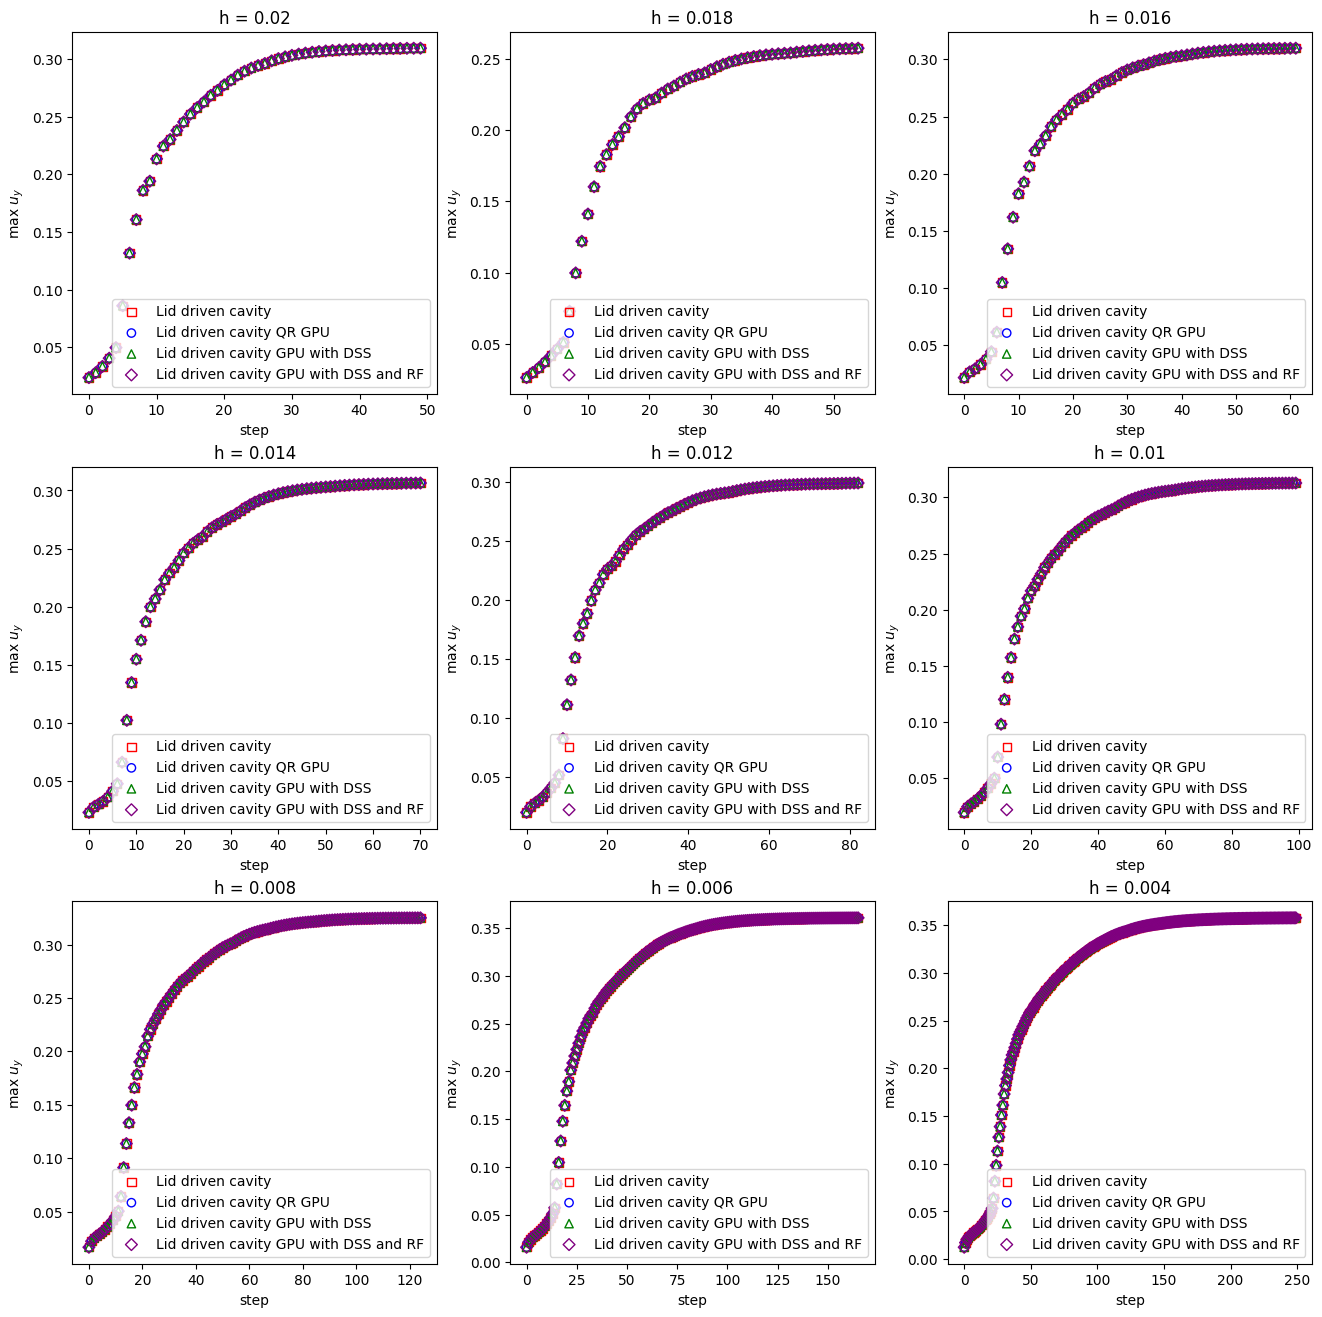
\includegraphics[width=0.8\textwidth]{lidDriven_convergence.png} 
    \caption{Graph of max $u_y$ in regard to number of steps taken using the implicit method.} 
    \label{fig:lidDriven_convergence} 
\end{figure}
\begin{figure}[h!] 
    \centering 
    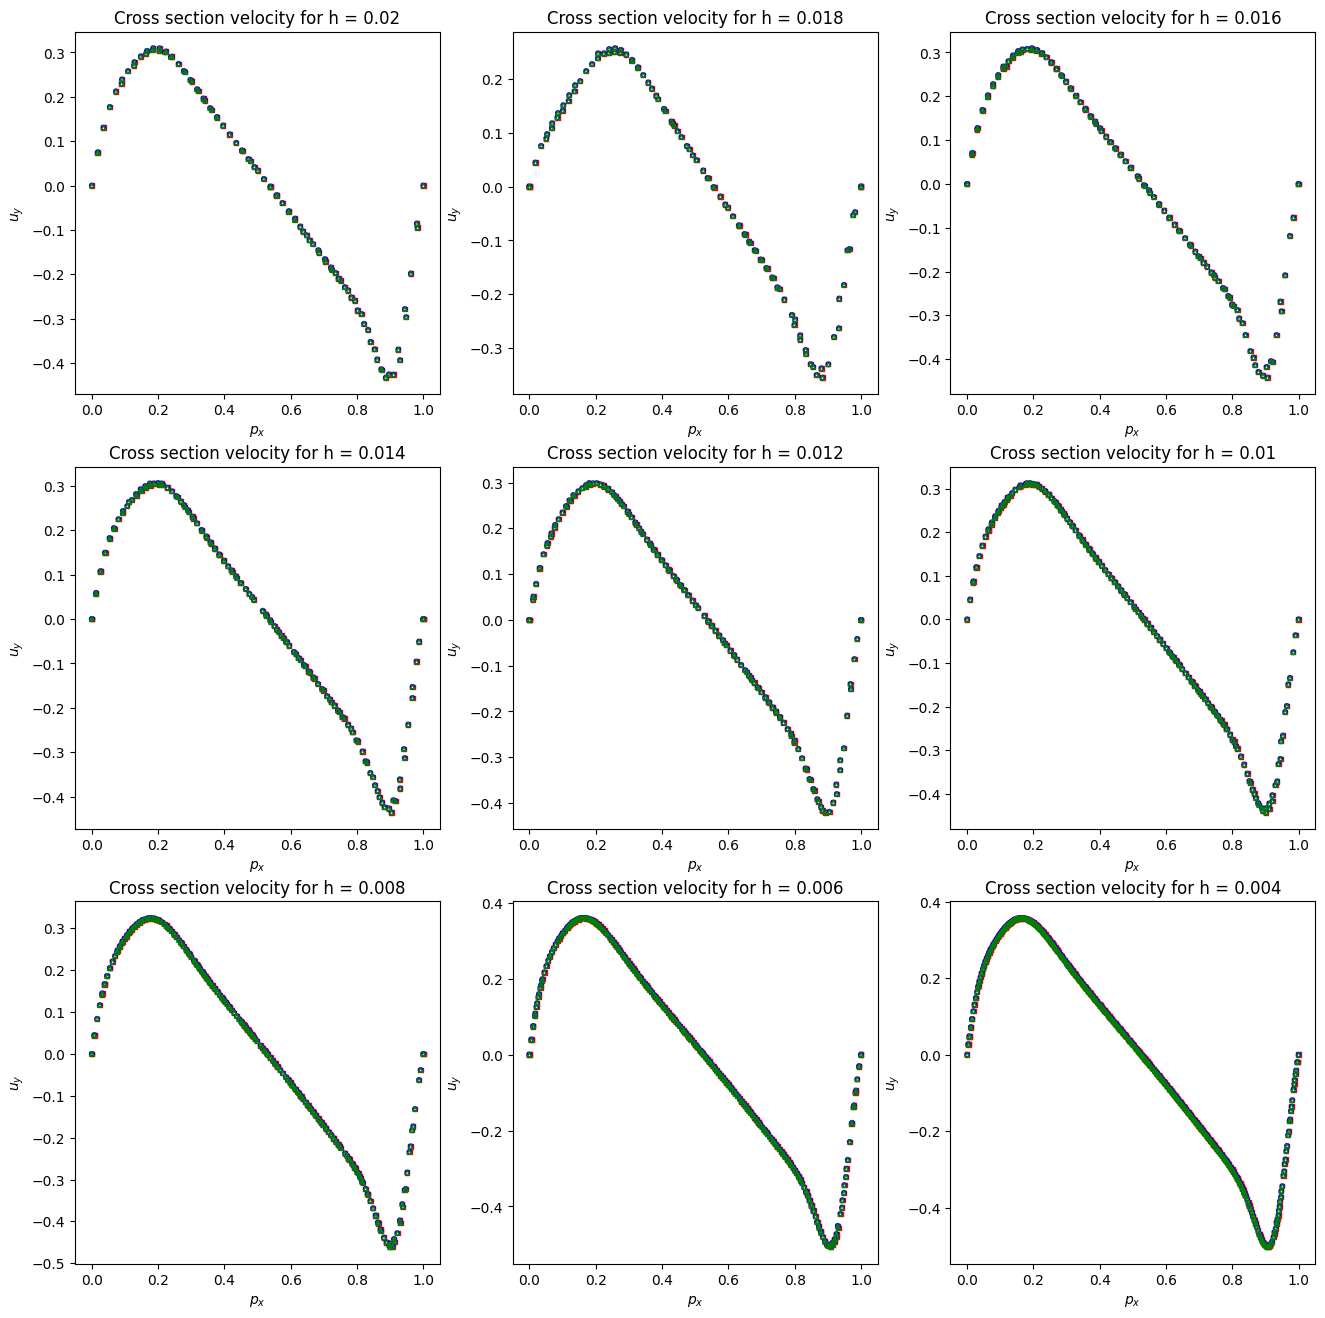
\includegraphics[width=0.8\textwidth]{lidDriven_cross.png} 
    \caption{Graph of velocities at the middle line after 50 seconds using the implicit method.} 
    \label{fig:lidDriven_cross} 
\end{figure}
\begin{figure}[h!] 
    \centering 
    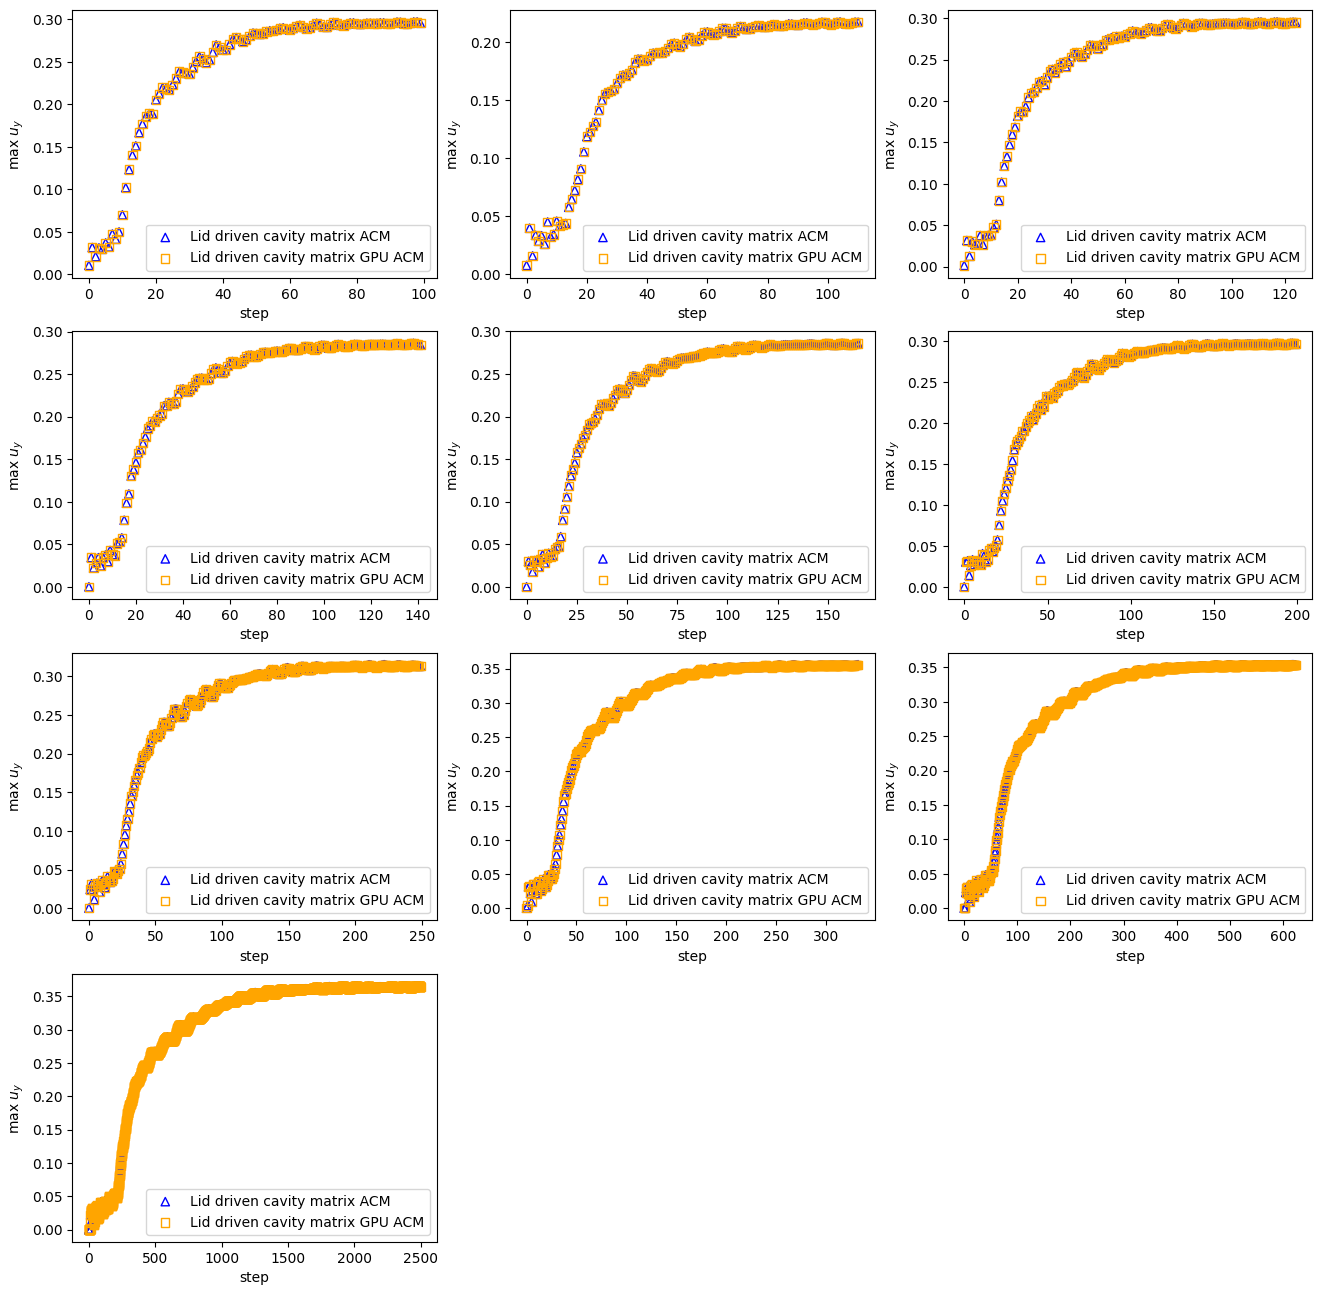
\includegraphics[width=0.8\textwidth]{lidDrivenACM_convergence.png} 
    \caption{Graph of max $u_y$ in regard to number of steps taken using the explicit method.} 
    \label{fig:lidDrivenACM_convergence} 
\end{figure}
\begin{figure}[h!] 
    \centering 
    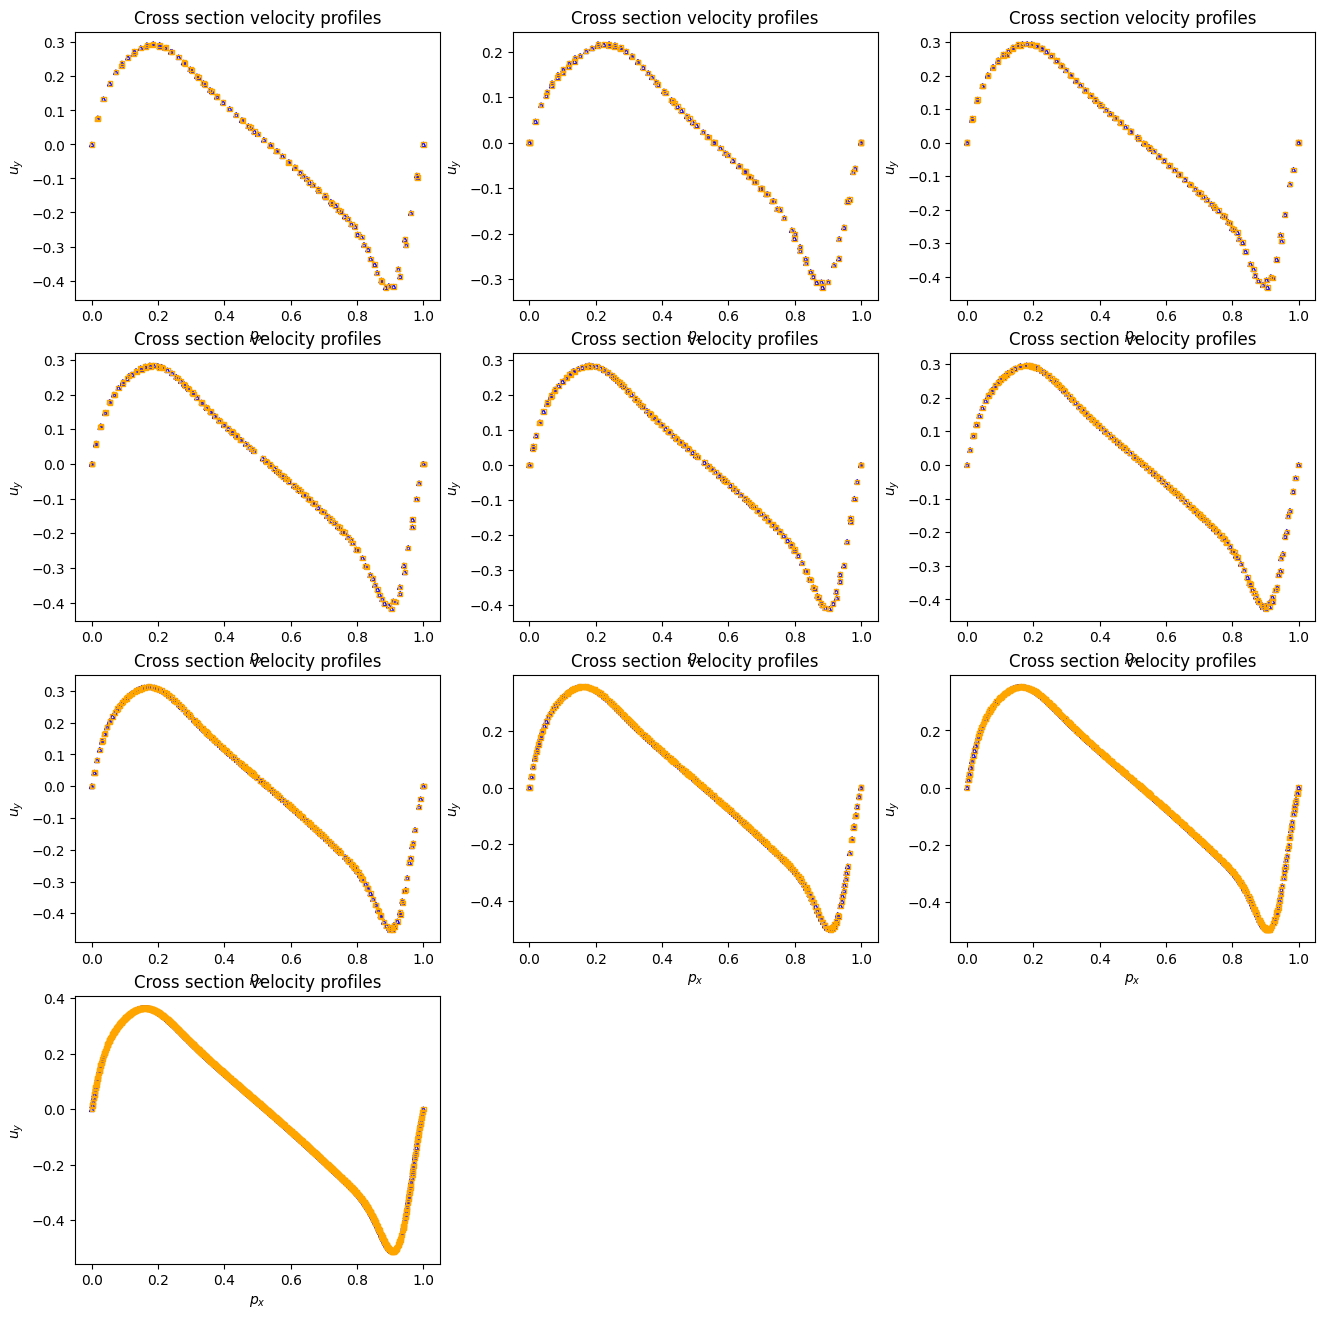
\includegraphics[width=0.8\textwidth]{lidDrivenACM_cross.png} 
    \caption{Graph of velocities at the middle line after 50 seconds using the explicit method.} 
    \label{fig:lidDrivenACM_cross} 
\end{figure}
\end{document}
